\section{eo\-NDSorting$<$ EOT $>$ Class Template Reference}
\label{classeo_n_d_sorting}\index{eoNDSorting@{eoNDSorting}}
Non dominated sorting, it $\ast$is a$\ast$ std::vector of doubles, the integer part is the rank (to which front it belongs), the fractional part the niching penalty or distance penalty or whatever penalty you want to squeeze into the bits.  


{\tt \#include $<$eo\-NDSorting.h$>$}

Inheritance diagram for eo\-NDSorting$<$ EOT $>$::\begin{figure}[H]
\begin{center}
\leavevmode
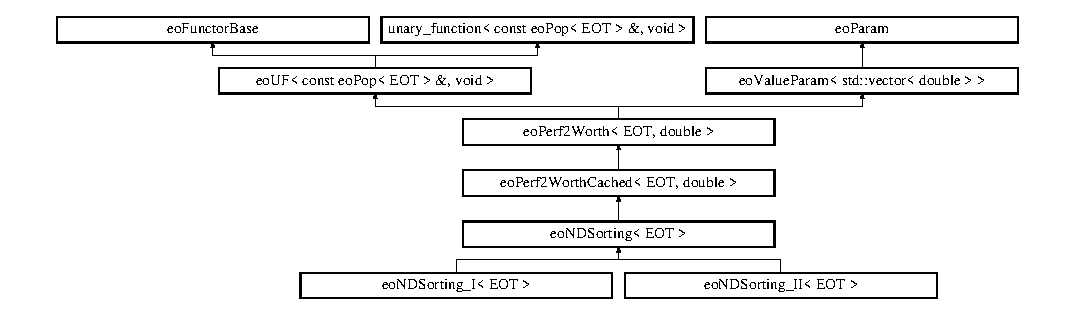
\includegraphics[height=3.78378cm]{classeo_n_d_sorting}
\end{center}
\end{figure}
\subsection*{Public Member Functions}
\begin{CompactItemize}
\item 
{\bf eo\-NDSorting} (bool nasty\_\-flag\_\-=false)\label{classeo_n_d_sorting_a0}

\item 
virtual std::vector$<$ double $>$ {\bf niche\_\-penalty} (const std::vector$<$ unsigned $>$ \&current\_\-front, const {\bf eo\-Pop}$<$ {\bf EOT} $>$ \&\_\-pop)=0
\begin{CompactList}\small\item\em Pure virtual function that calculates the 'distance' for each element in the current front Implement to create your own nondominated sorting algorithm. \item\end{CompactList}\item 
void {\bf calculate\_\-worths} (const {\bf eo\-Pop}$<$ {\bf EOT} $>$ \&\_\-pop)\label{classeo_n_d_sorting_a3}

\begin{CompactList}\small\item\em The actual virtual function the derived classes should implement. \item\end{CompactList}\end{CompactItemize}
\subsection*{Public Attributes}
\begin{CompactItemize}
\item 
bool {\bf nasty\_\-declone\_\-flag\_\-that\_\-only\_\-is\_\-implemented\_\-for\_\-two\_\-objectives}\label{classeo_n_d_sorting_o0}

\end{CompactItemize}
\subsection*{Private Member Functions}
\begin{CompactItemize}
\item 
void {\bf one\_\-objective} (const {\bf eo\-Pop}$<$ {\bf EOT} $>$ \&\_\-pop)\label{classeo_n_d_sorting_d0}

\item 
void {\bf two\_\-objectives} (const {\bf eo\-Pop}$<$ {\bf EOT} $>$ \&\_\-pop)
\begin{CompactList}\small\item\em Optimization for two objectives. \item\end{CompactList}\item 
void {\bf m\_\-objectives} (const {\bf eo\-Pop}$<$ {\bf EOT} $>$ \&\_\-pop)\label{classeo_n_d_sorting_d2}

\item 
void {\bf rank\_\-to\_\-worth} ()\label{classeo_n_d_sorting_d3}

\end{CompactItemize}


\subsection{Detailed Description}
\subsubsection*{template$<$class EOT$>$ class eo\-NDSorting$<$ EOT $>$}

Non dominated sorting, it $\ast$is a$\ast$ std::vector of doubles, the integer part is the rank (to which front it belongs), the fractional part the niching penalty or distance penalty or whatever penalty you want to squeeze into the bits. 



Definition at line 42 of file eo\-NDSorting.h.

\subsection{Member Function Documentation}
\index{eoNDSorting@{eo\-NDSorting}!niche_penalty@{niche\_\-penalty}}
\index{niche_penalty@{niche\_\-penalty}!eoNDSorting@{eo\-NDSorting}}
\subsubsection{\setlength{\rightskip}{0pt plus 5cm}template$<$class EOT$>$ virtual std::vector$<$double$>$ {\bf eo\-NDSorting}$<$ {\bf EOT} $>$::niche\_\-penalty (const std::vector$<$ unsigned $>$ \& {\em current\_\-front}, const {\bf eo\-Pop}$<$ {\bf EOT} $>$ \& {\em \_\-pop})\hspace{0.3cm}{\tt  [pure virtual]}}\label{classeo_n_d_sorting_a2}


Pure virtual function that calculates the 'distance' for each element in the current front Implement to create your own nondominated sorting algorithm. 

The size of the returned std::vector should be equal to the size of the current\_\-front. 

Implemented in {\bf eo\-NDSorting\_\-I$<$ EOT $>$} {\rm (p.\,\pageref{classeo_n_d_sorting___i_a1})}, and {\bf eo\-NDSorting\_\-II$<$ EOT $>$} {\rm (p.\,\pageref{classeo_n_d_sorting___i_i_a1})}.

Referenced by eo\-NDSorting$<$ EOT $>$::two\_\-objectives().\index{eoNDSorting@{eo\-NDSorting}!two_objectives@{two\_\-objectives}}
\index{two_objectives@{two\_\-objectives}!eoNDSorting@{eo\-NDSorting}}
\subsubsection{\setlength{\rightskip}{0pt plus 5cm}template$<$class EOT$>$ void {\bf eo\-NDSorting}$<$ {\bf EOT} $>$::two\_\-objectives (const {\bf eo\-Pop}$<$ {\bf EOT} $>$ \& {\em \_\-pop})\hspace{0.3cm}{\tt  [inline, private]}}\label{classeo_n_d_sorting_d1}


Optimization for two objectives. 

Makes the algorithm run in complexity O(n log n) where n is the population size

This is the same complexity as for a single objective or truncation selection or sorting.

It will perform a sort on the two objectives seperately, and from the information on the ranks of the individuals on these two objectives, the non-dominated sorting rank is determined. There are then three nlogn operations in place: one sort per objective, plus a binary search procedure to combine the information about the ranks.

After that it is a simple exercise to calculate the distance penalty 

Definition at line 140 of file eo\-NDSorting.h.

References eo\-NDSorting$<$ EOT $>$::niche\_\-penalty(), and eo\-Value\-Param$<$ std::vector$<$ double $>$ $>$::value().

Referenced by eo\-NDSorting$<$ EOT $>$::calculate\_\-worths().

The documentation for this class was generated from the following file:\begin{CompactItemize}
\item 
eo\-NDSorting.h\end{CompactItemize}
